\begin{figure}
  \begin{subfigure}{0.24\linewidth}
    \centering
    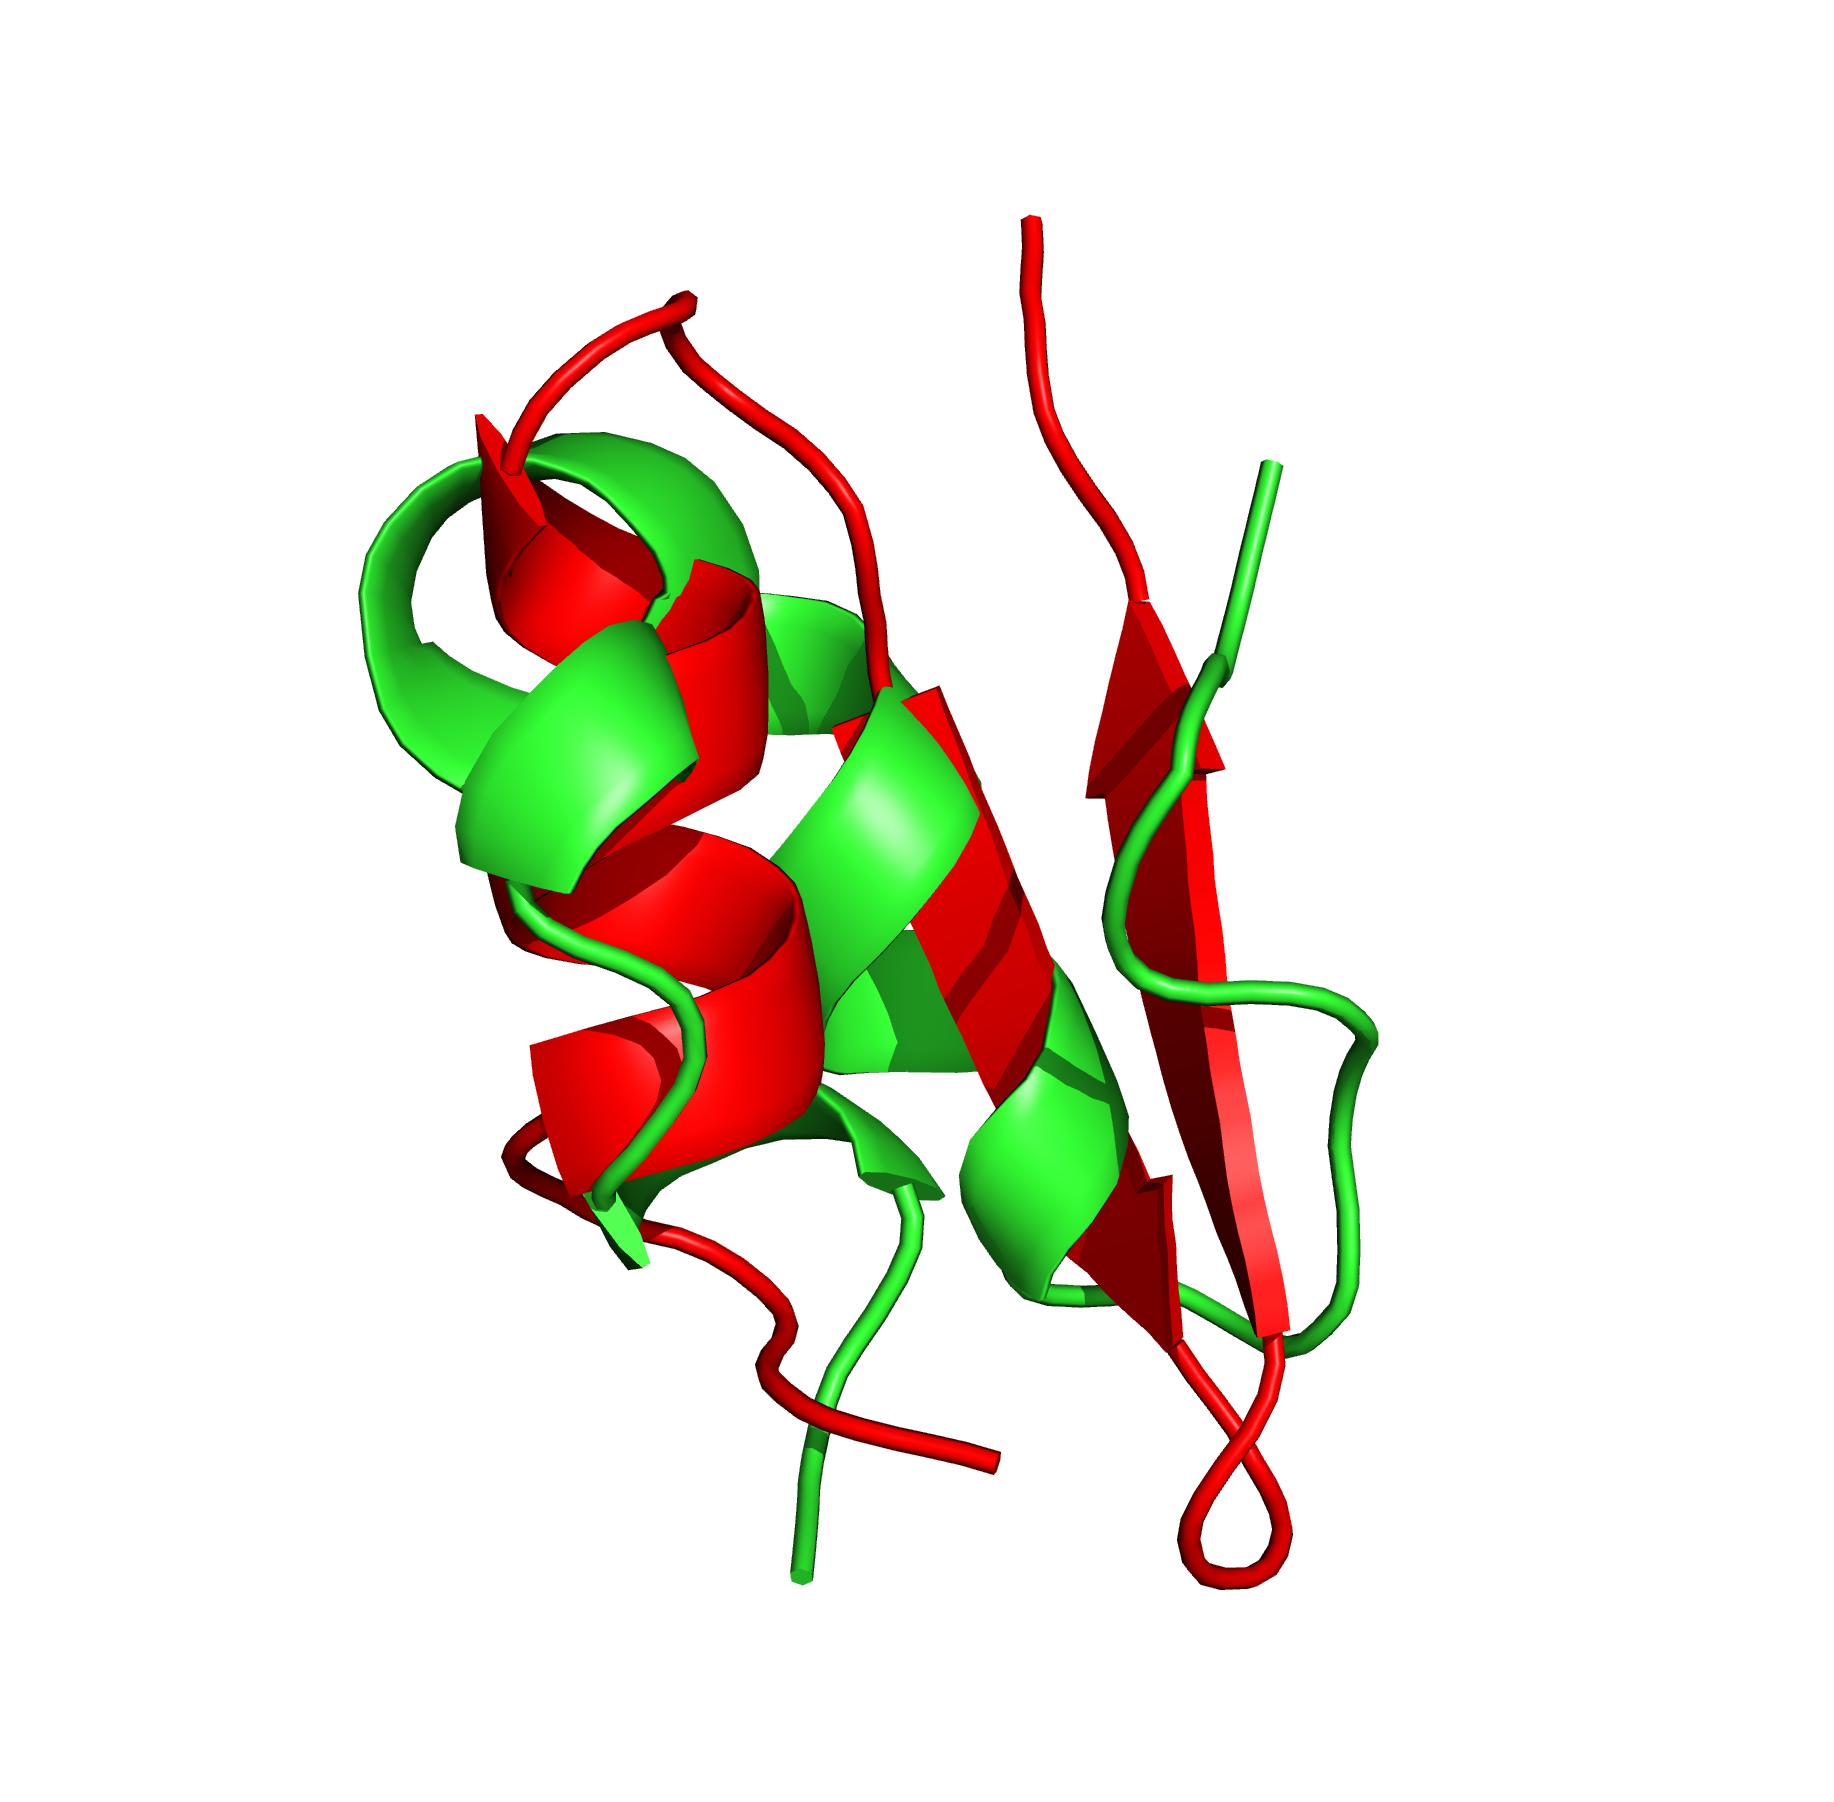
\includegraphics[width=0.9\linewidth]{Figuras/prots/1acw_render.png}
    \caption{1acw}
    \label{fig:1acw-conformation}
  \end{subfigure}
%
  \begin{subfigure}{0.24\linewidth}
    \centering
    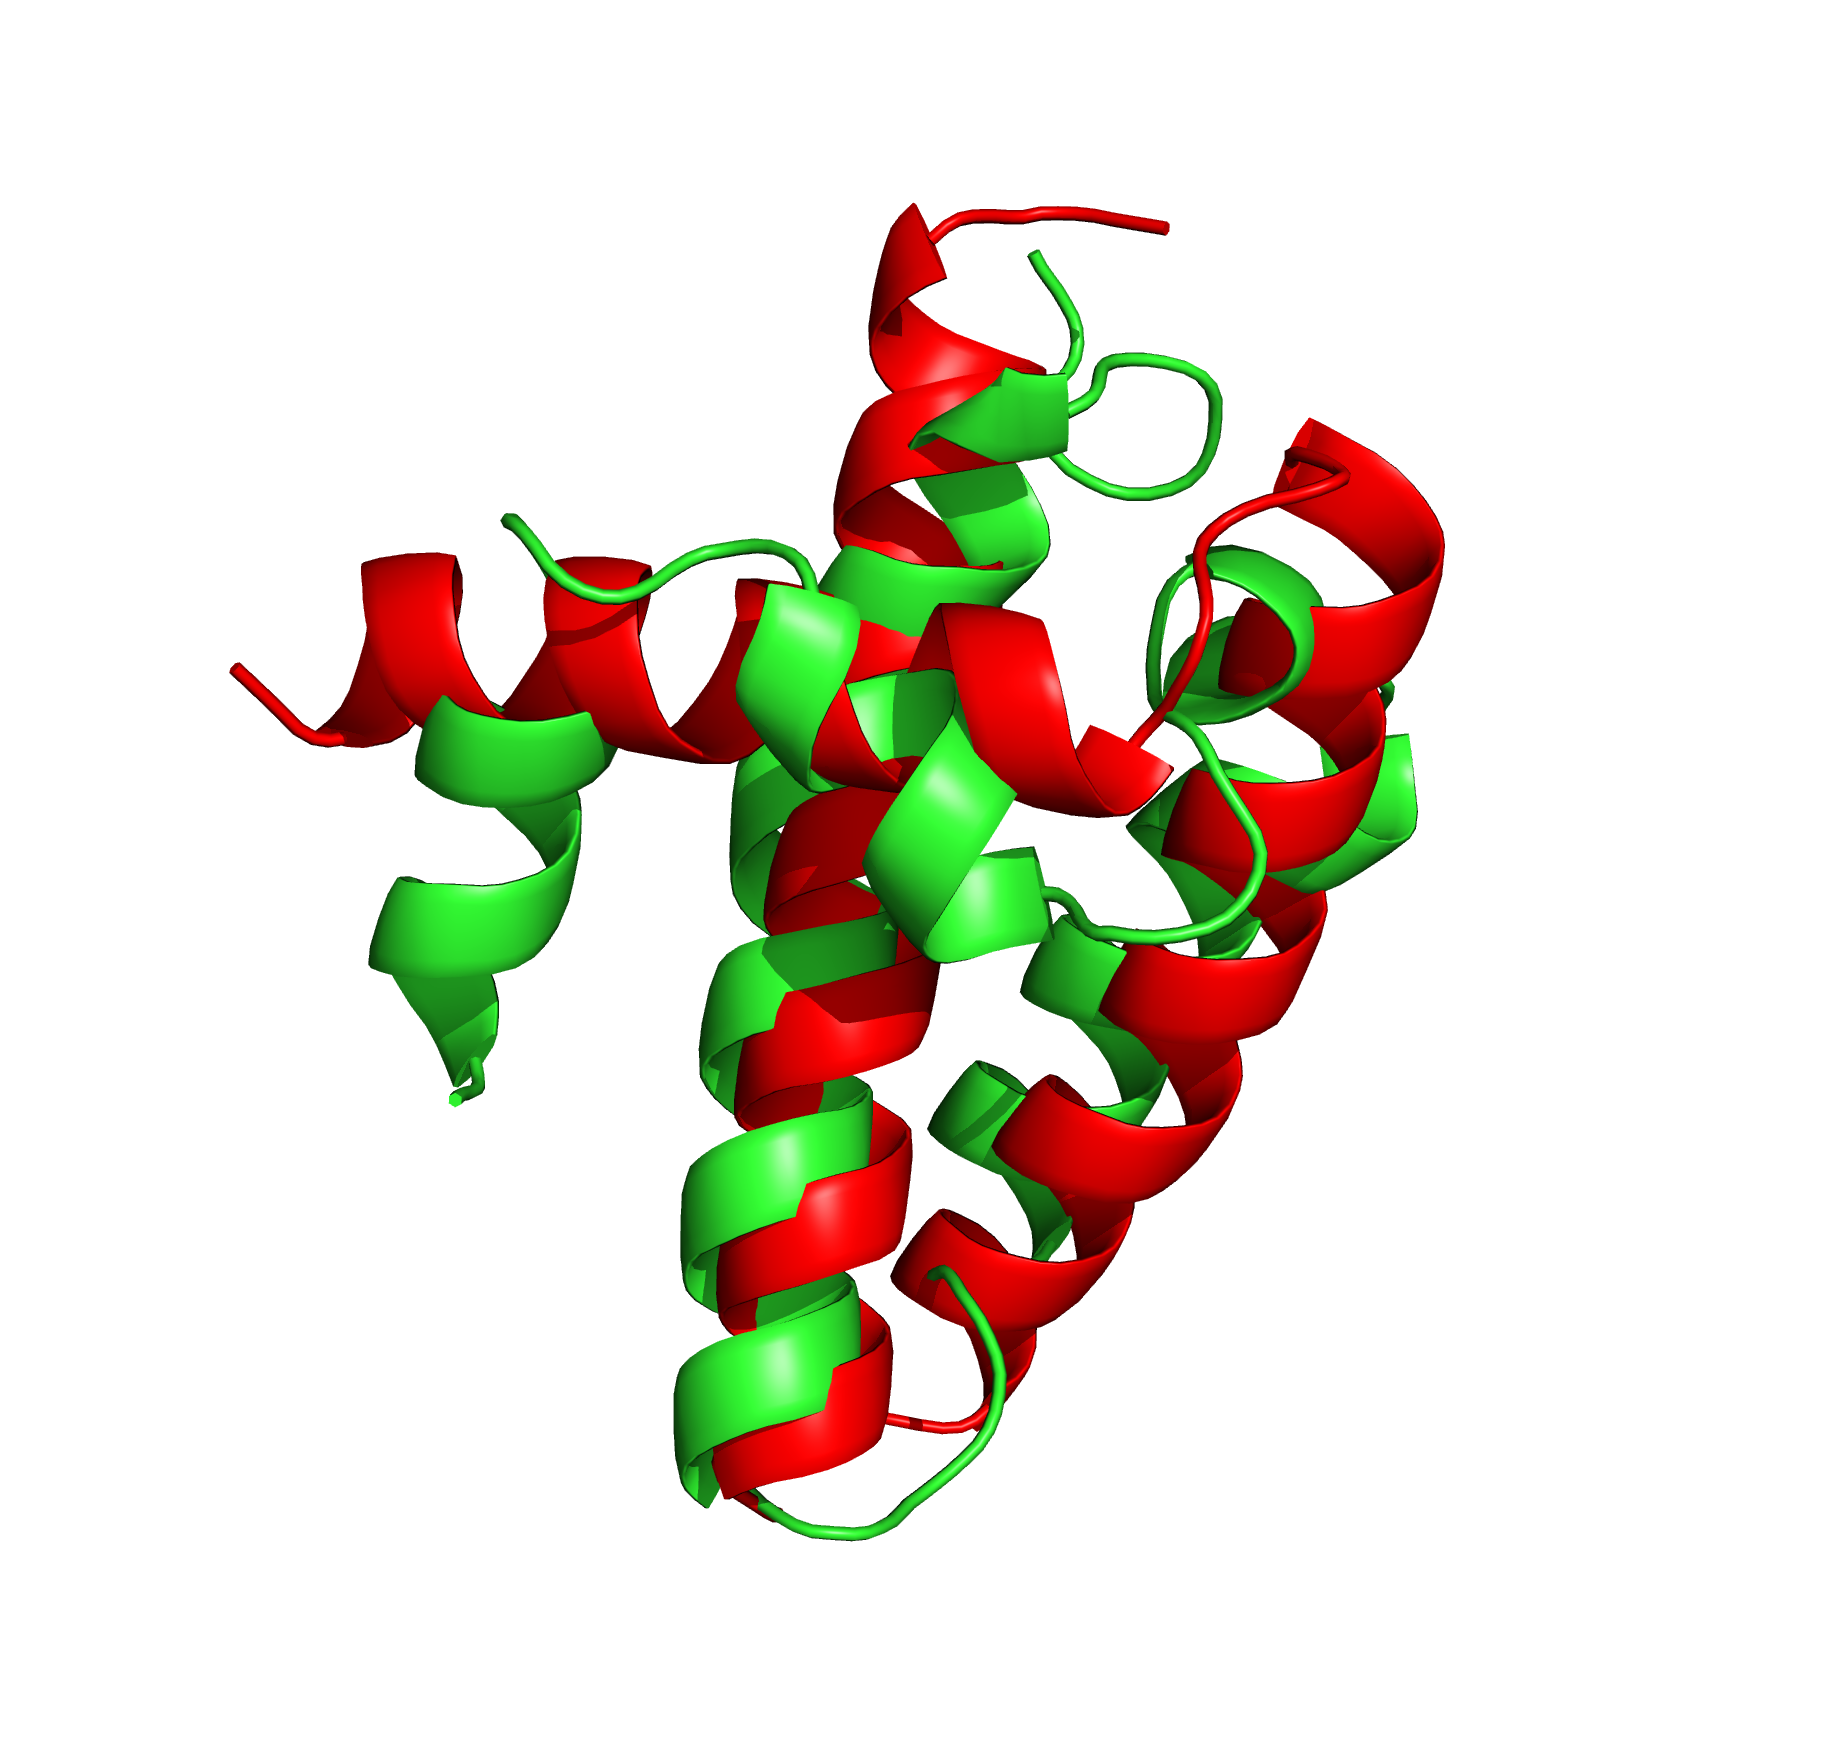
\includegraphics[width=0.9\linewidth]{Figuras/prots/1ail_render.png}
    \caption{1ail}
    \label{fig:1ail-conformation}
  \end{subfigure}
%
  \begin{subfigure}{0.24\linewidth}
    \centering
    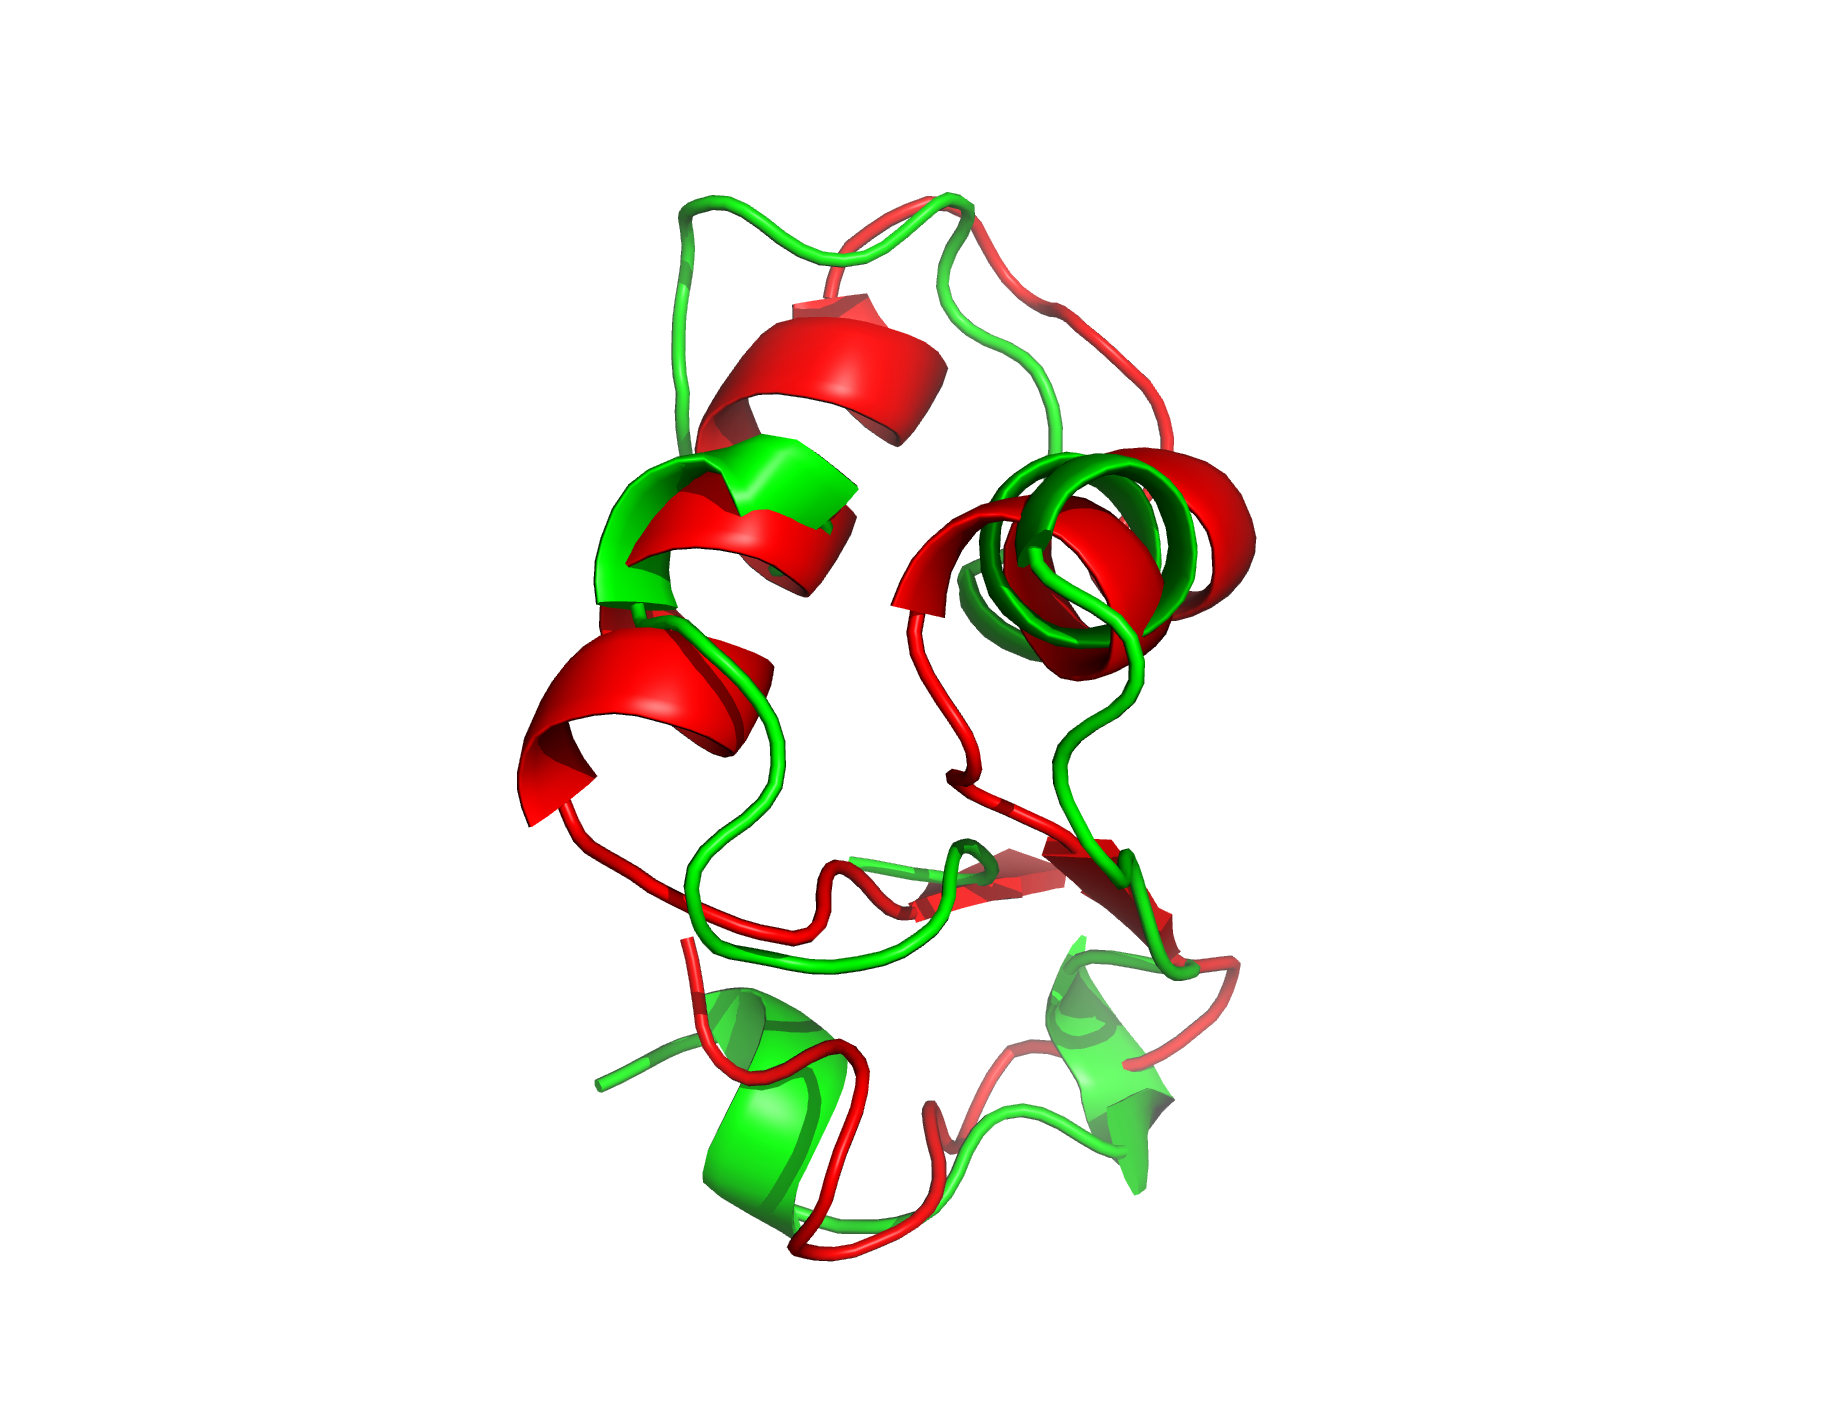
\includegraphics[width=0.9\linewidth]{Figuras/prots/1crn_render.png}
    \caption{1crn}
    \label{fig:1crn-conformation}
  \end{subfigure}
%
  \begin{subfigure}{0.24\linewidth}
    \centering
    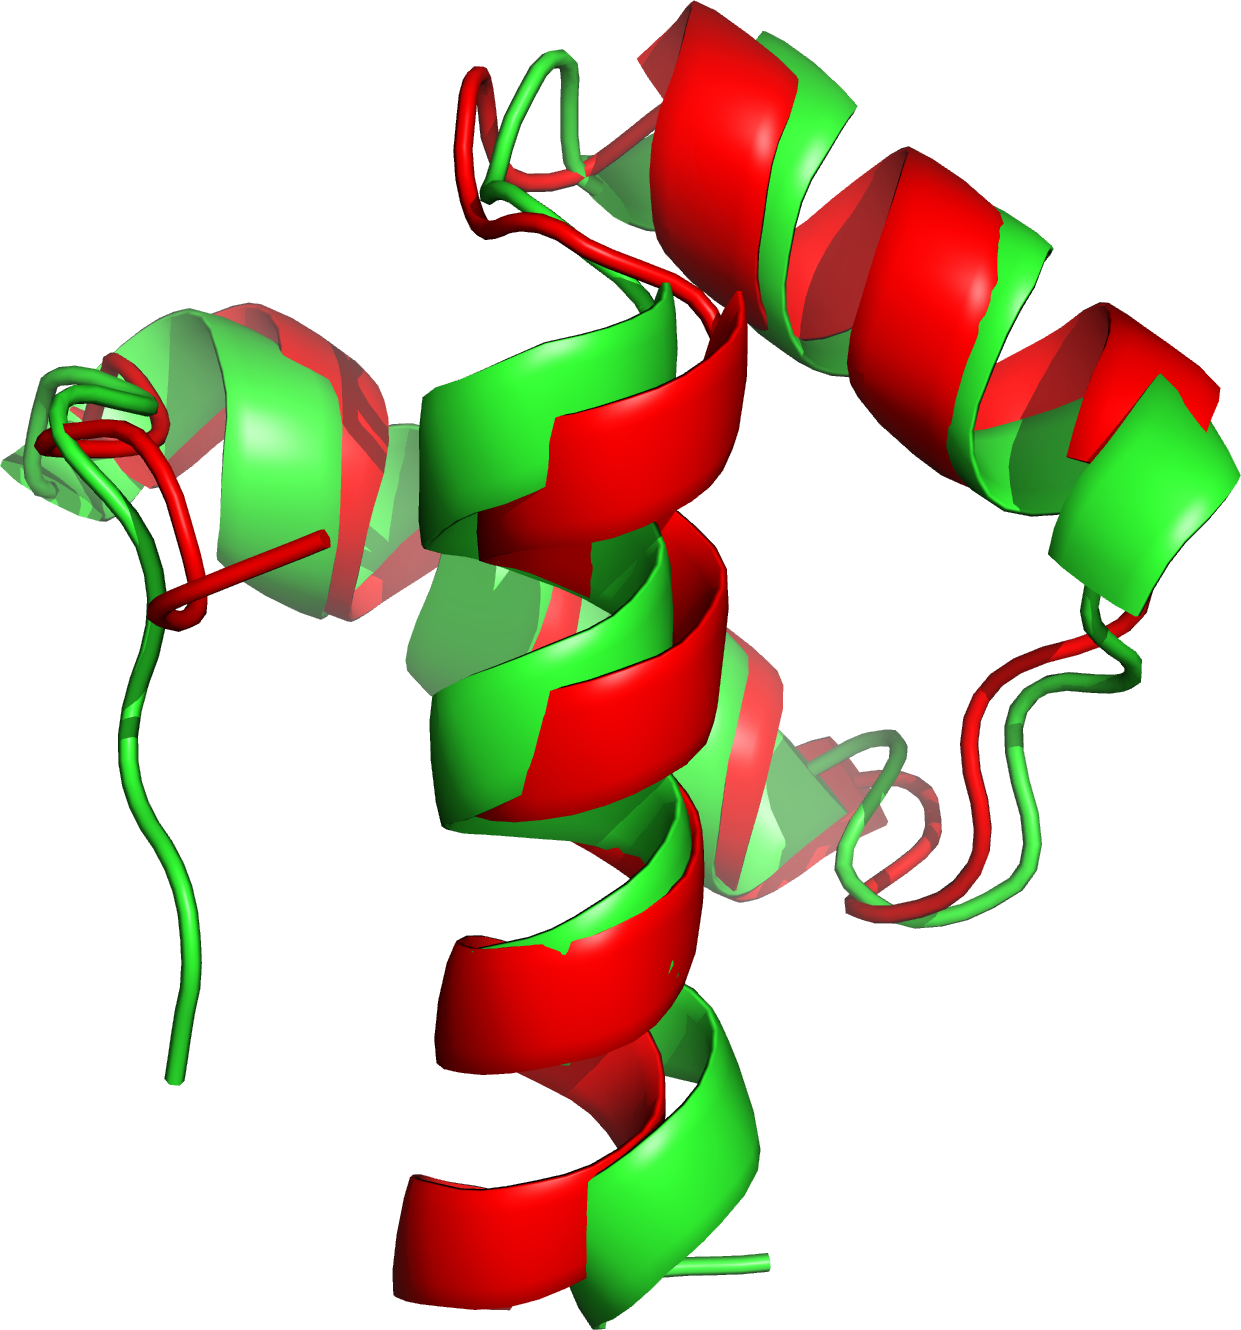
\includegraphics[width=0.9\linewidth]{Figuras/prots/1enh_render.png}
    \caption{1enh}
    \label{fig:1enh-conformation}
  \end{subfigure}
% \end{figure}
% \begin{figure}
  \begin{subfigure}{0.32\linewidth}
    \centering
    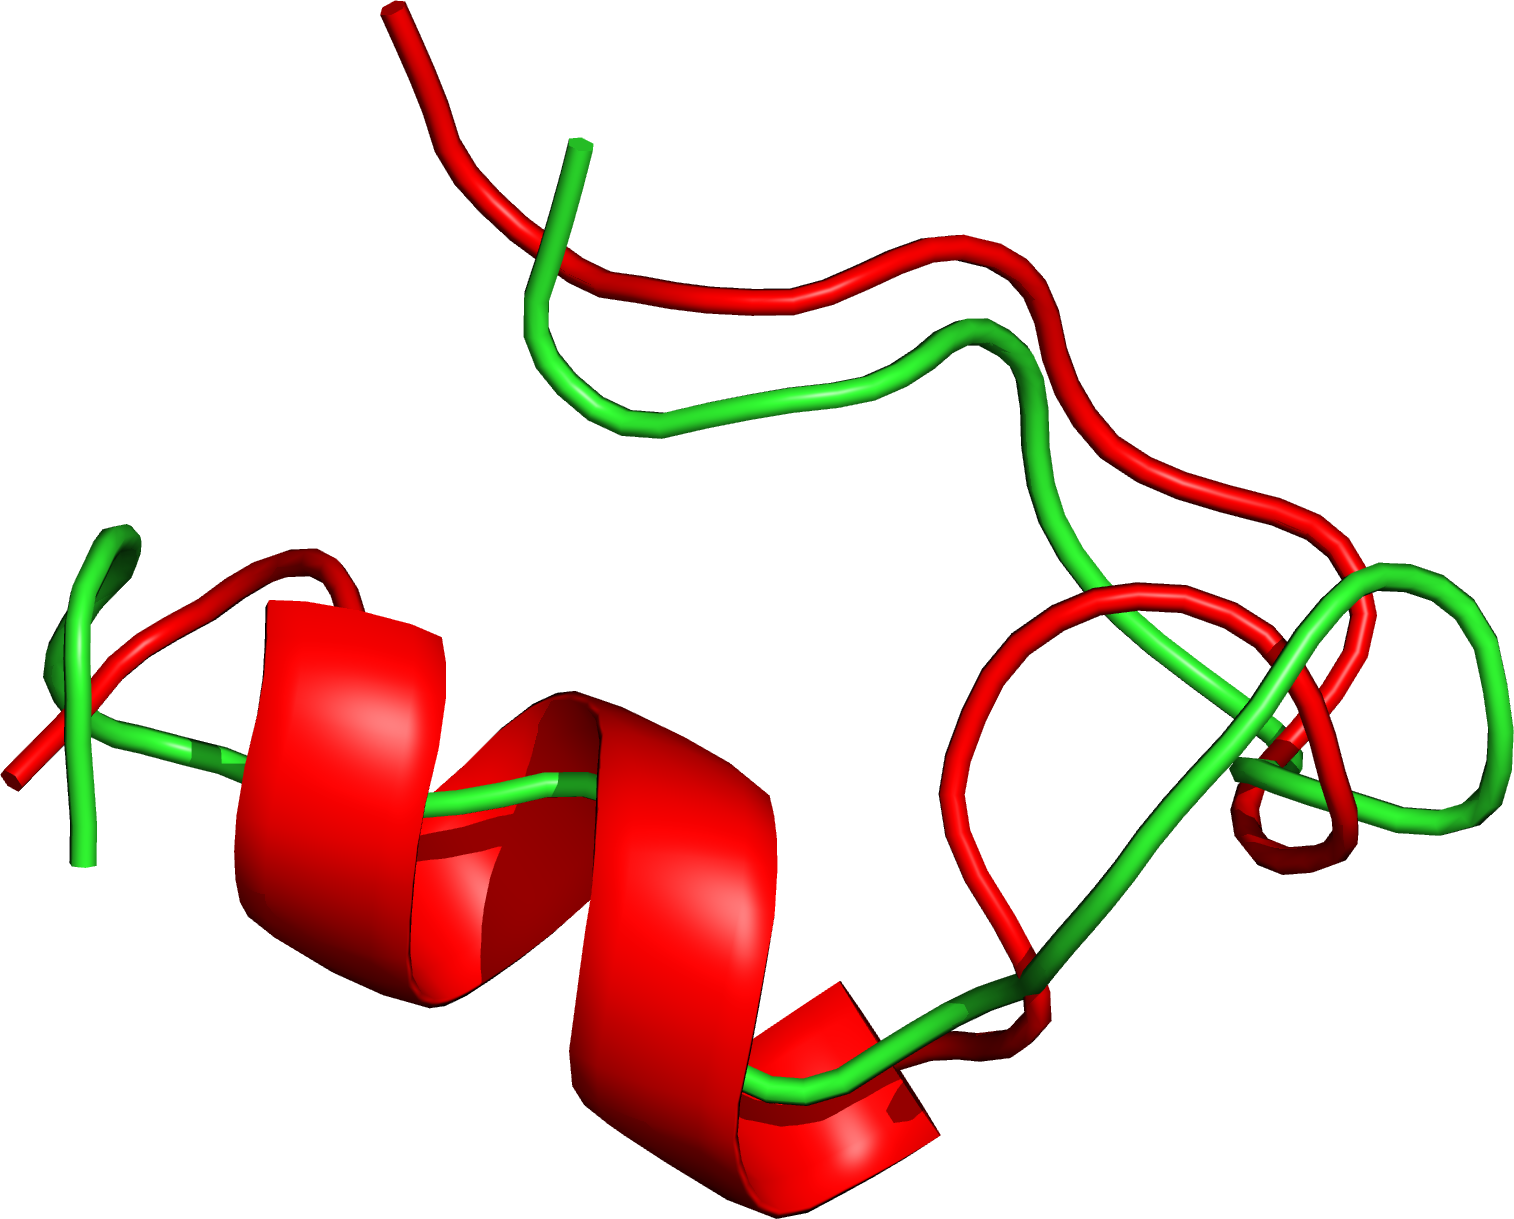
\includegraphics[width=0.9\linewidth]{Figuras/prots/1l2y_render.png}
    \caption{1l2y}
    \label{fig:1l2y-conformation}
  \end{subfigure}
%
  \begin{subfigure}{0.32\linewidth}
    \centering
    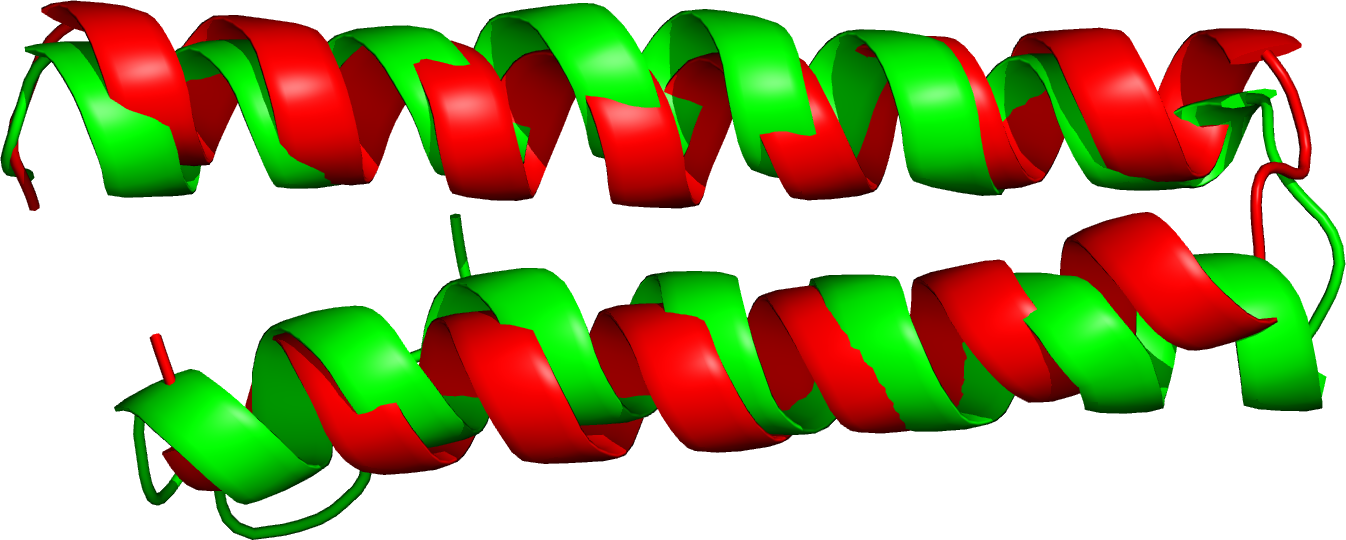
\includegraphics[width=0.9\linewidth]{Figuras/prots/1rop_render.png}
    \caption{1rop}
    \label{fig:1rop-conformation}
  \end{subfigure}
%
  \begin{subfigure}{0.32\linewidth}
    \centering
    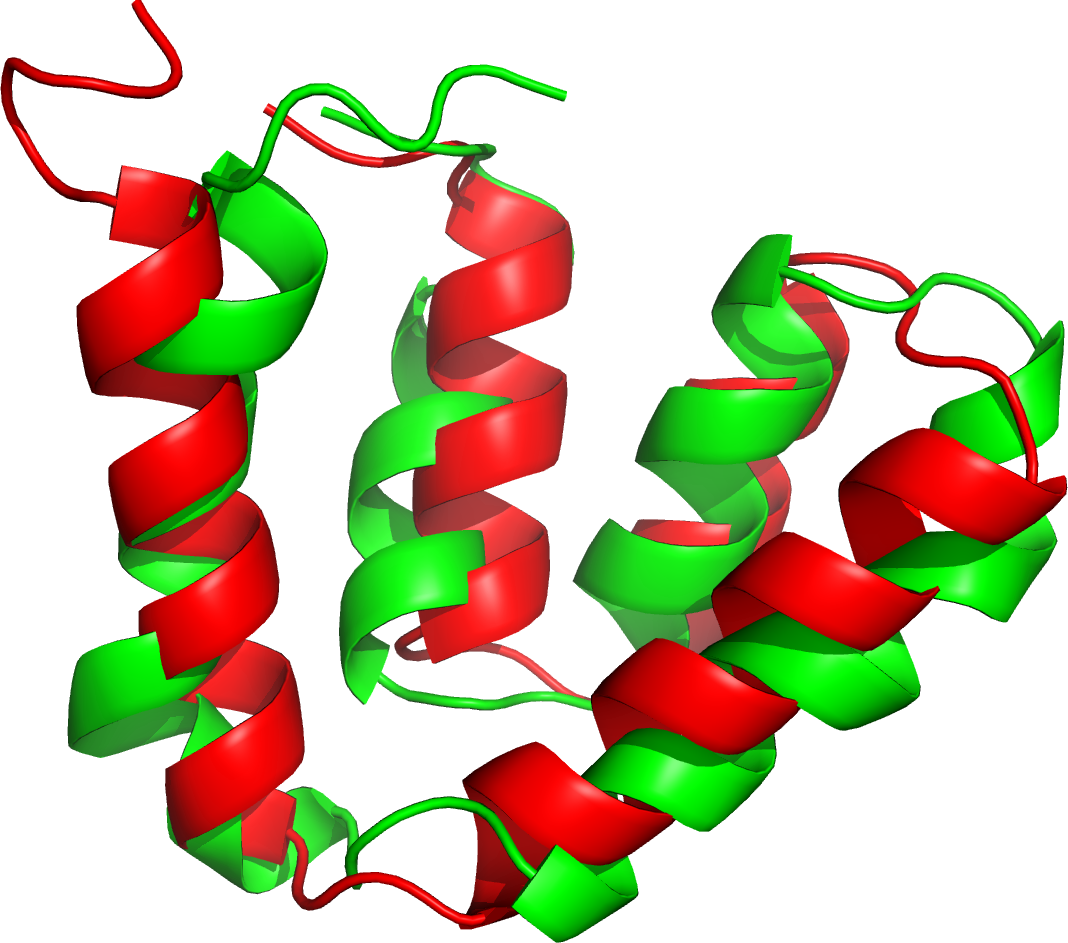
\includegraphics[width=0.9\linewidth]{Figuras/prots/1utg_render.png}
    \caption{1utg}
    \label{fig:1utg-conformation}
  \end{subfigure}
% \end{figure}
% \begin{figure}
  \begin{subfigure}{0.32\linewidth}
    \centering
    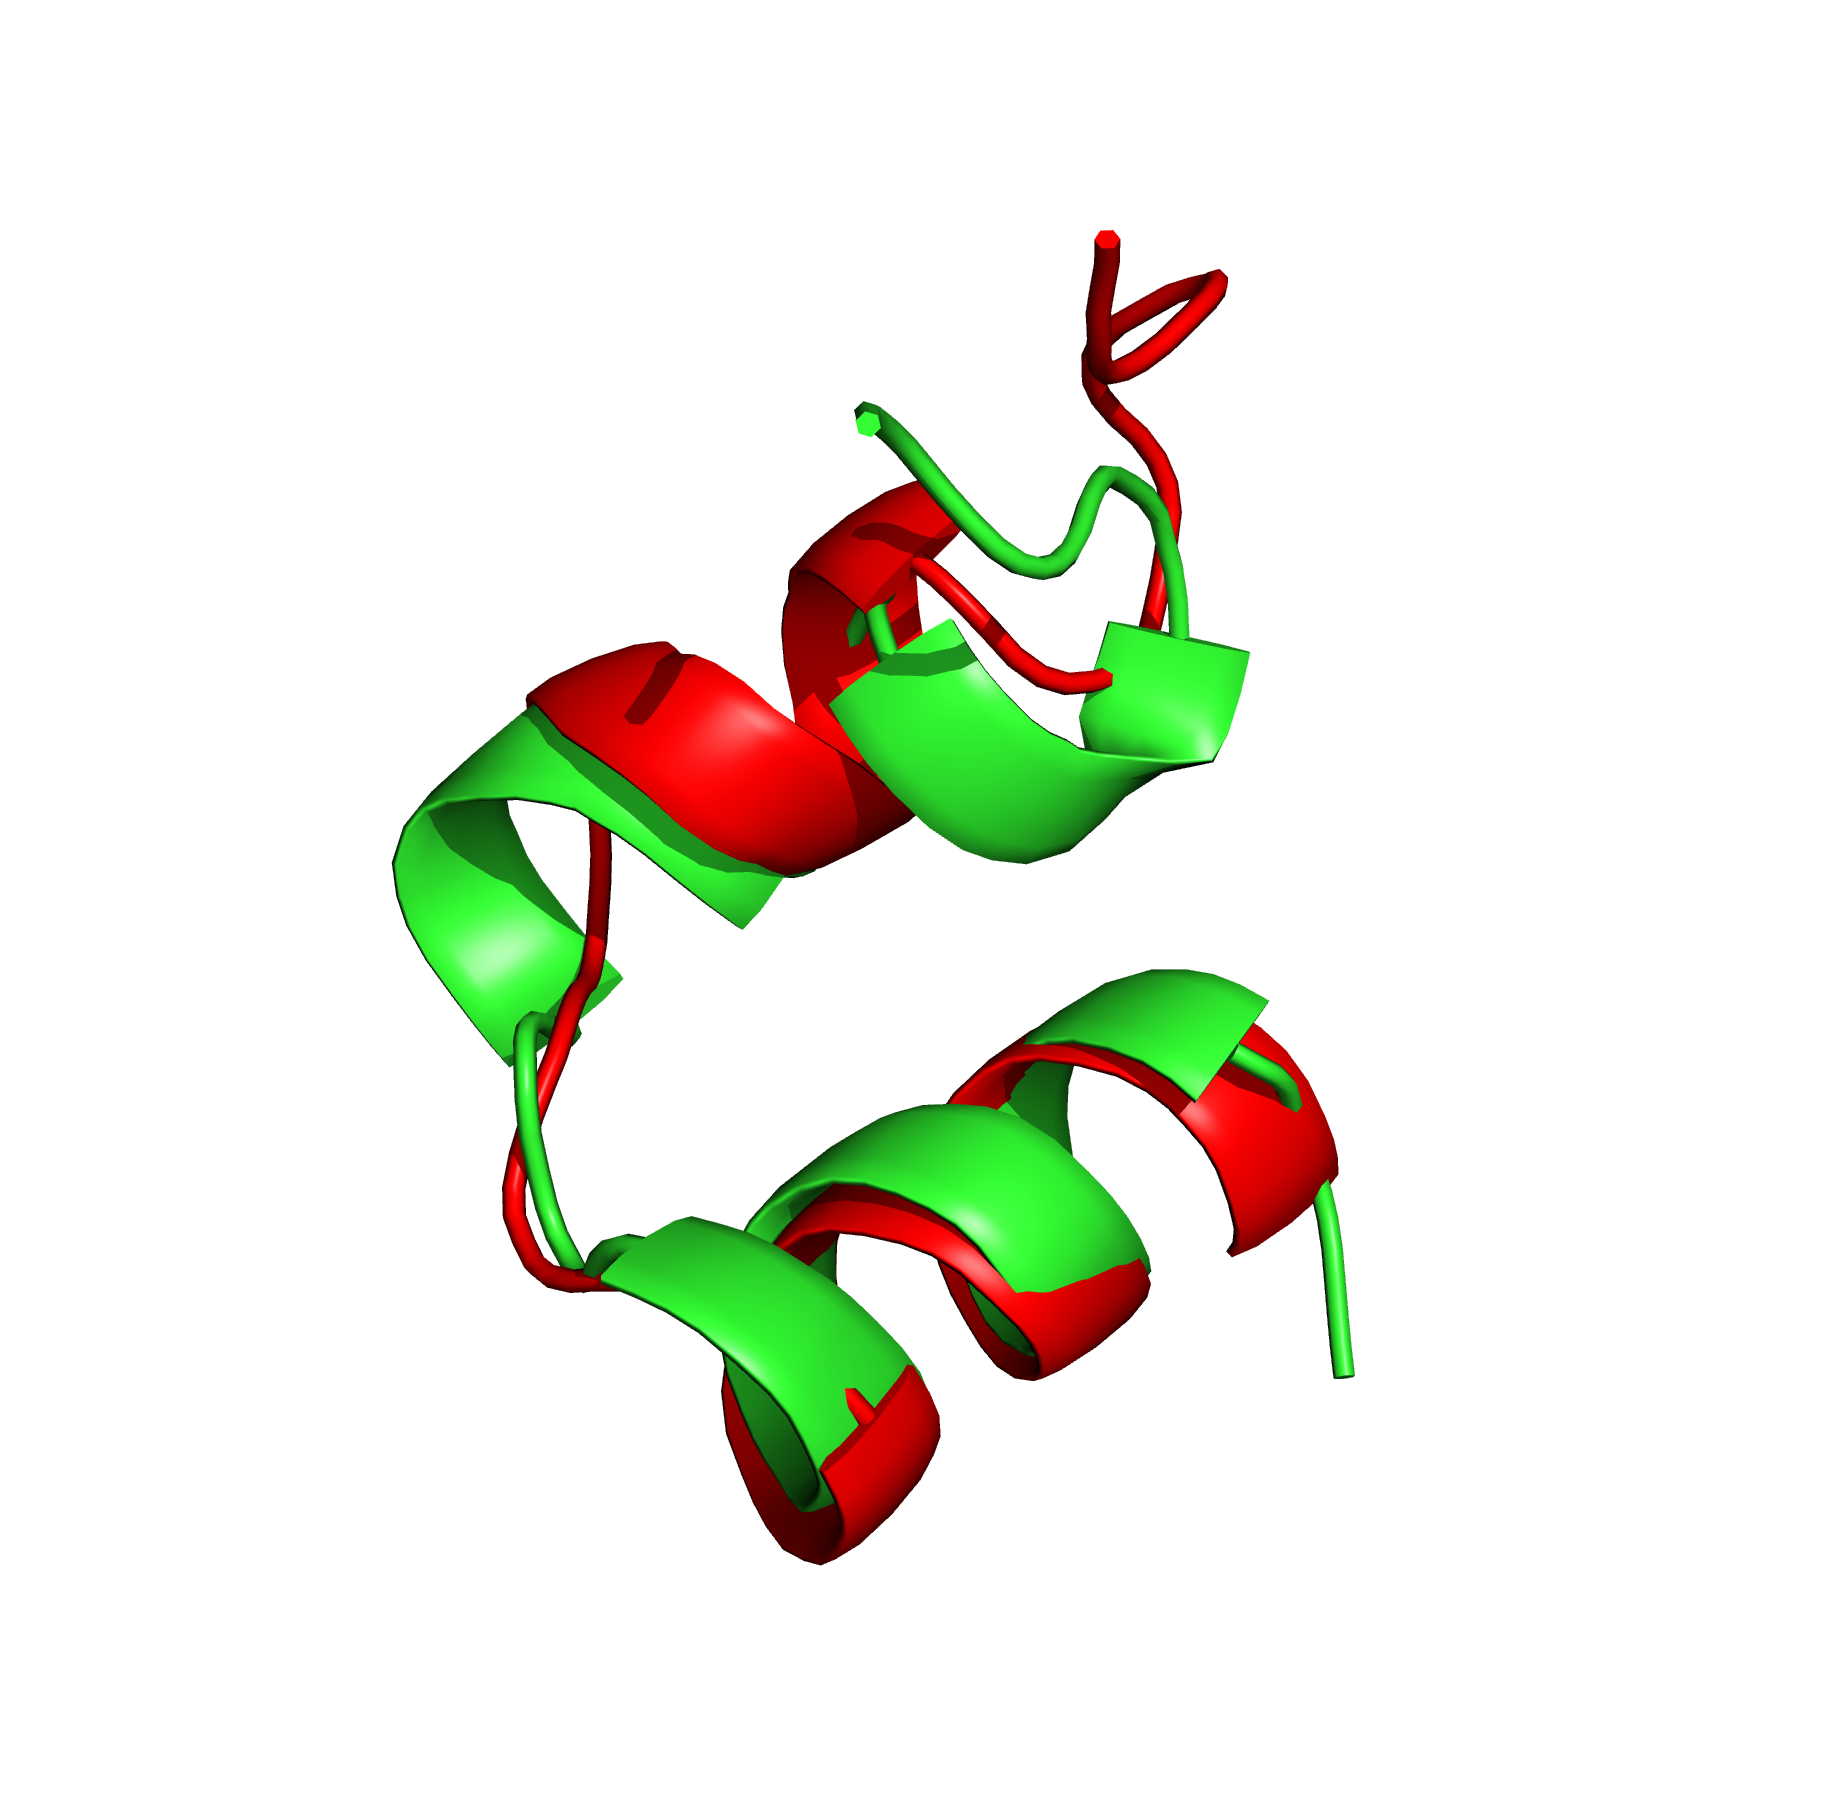
\includegraphics[width=0.9\linewidth]{Figuras/prots/1wqc_render.png}
    \caption{1wqc}
    \label{fig:1wqc-conformation}
  \end{subfigure}
%
  \begin{subfigure}{0.32\linewidth}
    \centering
    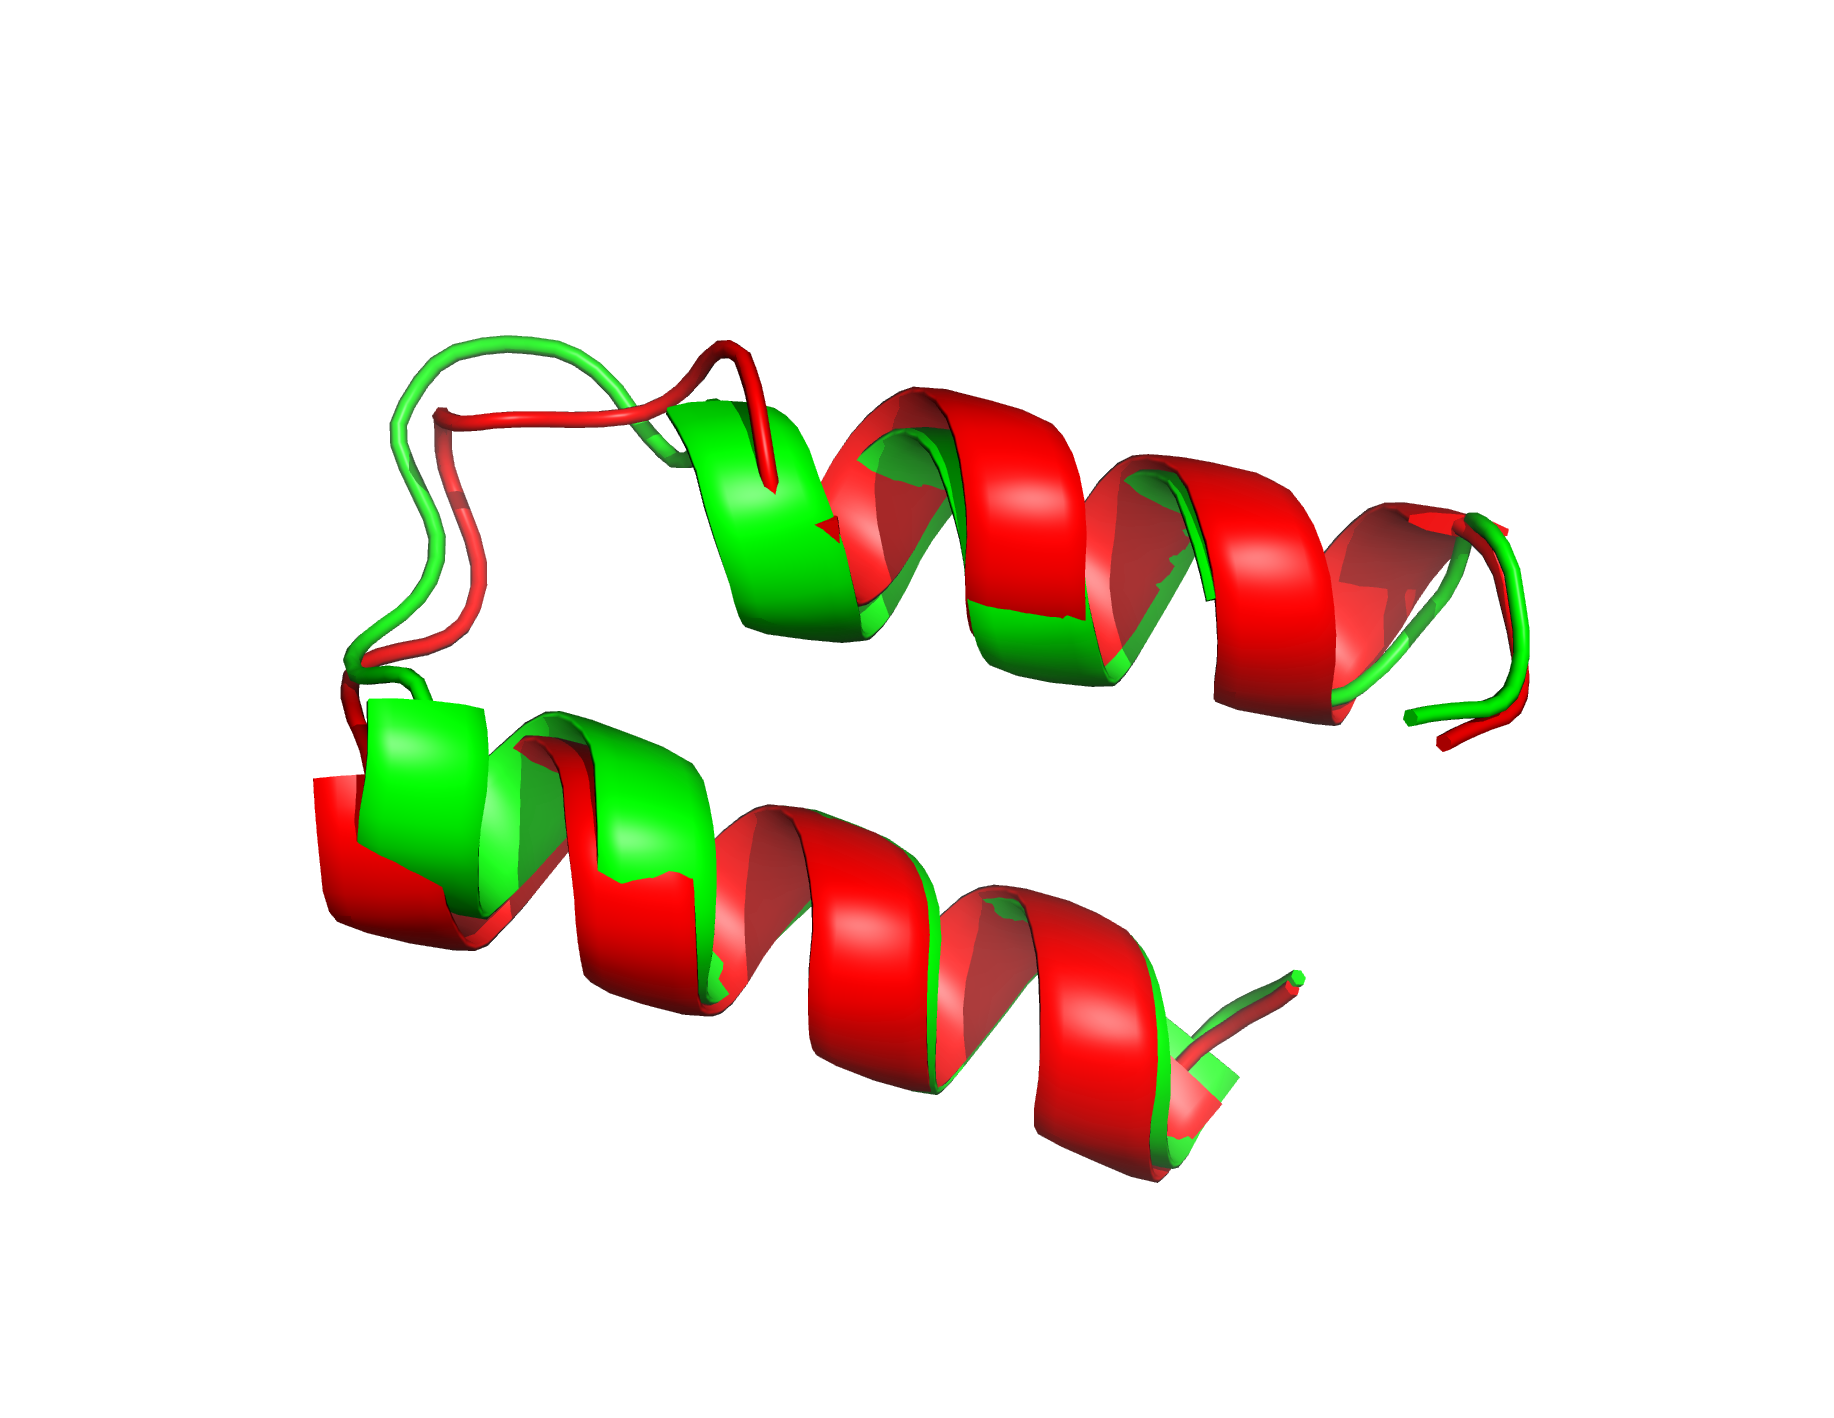
\includegraphics[width=0.9\linewidth]{Figuras/prots/1zdd_render.png}
    \caption{1zdd}
    \label{fig:1zdd-conformation}
  \end{subfigure}
%
  \begin{subfigure}{0.32\linewidth}
    \centering
    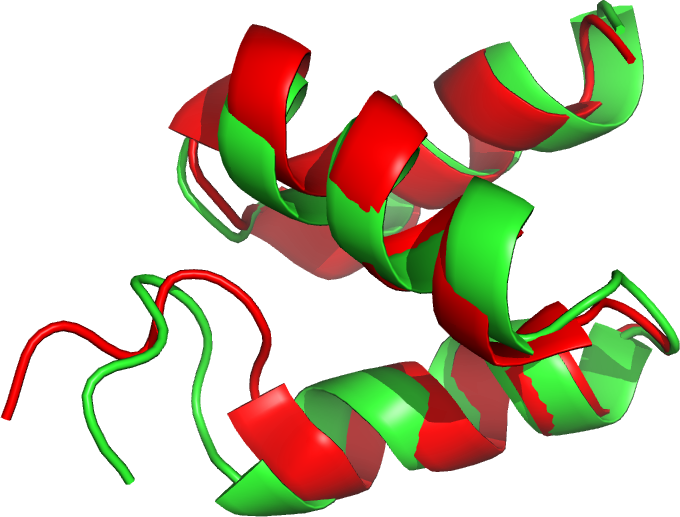
\includegraphics[width=0.9\linewidth]{Figuras/prots/2mr9_render.png}
    \caption{2mr9}
    \label{fig:2mr9-conformation}
  \end{subfigure}
  \caption{The predicted conformations (in green/light gray) compared to the
  native conformation (in red/darker gray)}
  \label{fig:all-conformations}
\end{figure}
